%TODO: is the problem real?
%TODO: Q-function or Q-value
%TODO: rigorous proof?
%TODO: format
%TODO: citation correct
%TODO: more reference
%TODO: line 171
%TODO: GLIE
%TODO: page 6 bottom
%TODO: Figure
%[1, 2], line 360
\documentclass{article} % For LaTeX2e
\usepackage{nips11submit_e,times}
%\documentstyle[nips10submit_09,times,art10]{article} % For LaTeX 2.09
\usepackage{graphicx} 


\RequirePackage{amsfonts}
\RequirePackage{amsmath}
\newtheorem{definition}{Definition}
\newtheorem{theorem}{Theorem}
\newtheorem{proof}{Proof}
\newtheorem{conjecture}{Conjecture}

\newcommand{\suchthat}{ \mathrel{\ooalign{$\ni$\cr\kern-1pt$-$\kern-6.5pt$-$}}}

\title{Optimal Planning with Approximate Model-Based Reinforcement Learning}


\author{
Hai-Feng Kao
Department of Computer Science\\
University of British Columbia\\
\texttt{haifeng@cs.ubc.ca}
}

% The \author macro works with any number of authors. There are two commands
% used to separate the names and addresses of multiple authors: \And and \AND.
%
% Using \And between authors leaves it to \LaTeX{} to determine where to break
% the lines. Using \AND forces a linebreak at that point. So, if \LaTeX{}
% puts 3 of 4 authors names on the first line, and the last on the second
% line, try using \AND instead of \And before the third author name.

\newcommand{\fix}{\marginpar{FIX}}
\newcommand{\new}{\marginpar{NEW}}

%\nipsfinalcopy % Uncomment for camera-ready version

\begin{document}


\maketitle

\begin{abstract}
Model-based reinforcement learning methods make efficient use of samples by 
building a model of the environment and planning with it.
Compared to model-free methods, they usually take fewer samples to converge to the optimal policy.
Despite that efficiency, model-based methods
need to enumerate all possible states during planning process,
thus it is impractical to apply model-based methods to large domains.
In this paper, we propose a simple approach that assumes most of the variables 
are static during the planning process and focuses on modeling the few dynamic variables.
By combining this approach with 
hierarchically optimal recursive Q-learning under 
a hierarchical reinforcement learning framework, we show that
the proposed approach learns the optimal policy even when
the assumptions of the model are not satisfied.
\end{abstract}


%contribution: if the approximated model is good, it will converge faster than flat SARSA. 
%if not, it still converge eventually
%model-based approach is hard, they cannot figure out the correct Q value because the design of the model is biased
%model-free is ok because Gt doesn't require a model
%A fail safe mechanism to ensure that approximated model-based approach may
%converge to optimal policy even when the model is approximated
%converge even when our model is biased
%if the model worked--> converge to optimal policy fast
%if not, it will converge to the optimal policy anyway
%1. Motivate the purpose: 
   %0. the factered model is intrinsticly biased for non factored one
   %1. the power of model based approach (introduce the previous work and the lack of approximation)
   %2. previous work on approximated model based approach (2 actions and n steps is O(2^n))
   %2. previous work on model-based HRL
   %3. previous work on hybrid approach (no guaranntee on a approximated model) (all coarse to fine approach)
   %4. introduce HORDQ
   %5. the problem of HORDQ: worse than flat Q without transfer, our sol: add internal reward
   %6. our contribution: show that the important property is that it will converge to optimal policy for any planner
   %7. our contribution: combine with model-based approach (HORDQ is userful when we combine it with some approximated model)
   %8. a natural extension: use high internal reward in the beginning and decrease it in the end
   %Hierarchical Policy Gradient Algorithms
%2. Introduction on MAXQ
%3. Biased model
%4. HORDQ
%4.1. Pseudo reward
%5. the leaf cover
%6. add all primitive actions and the necessary (and the price)
%5. show the optimality
%5.1. the offline case (not depend on Andre's proof)
%5.2. the online case (the conjecture status, how about chaning policy (value iteration)? --> define a new mdp)
%5.3. TD equation
%6. The three optimality (recursive optimality is not possible(model is approximated) bottom node recursive optimal is bad (always select get passenger),hierarchical optimality is impossible. the only hope is optimal)
%7. the respect of the hierarchy
%8. The experiment (school bus problem)
%9. The optimality cannot be achieved with recursive optimal (random planner with MAXQ --> the problem of existing approximation approach)
%10. With HORDQ, it is possible but slow (random planner with HORDQ)
%11. with appropriate penality it can be faster
%12. it works well if sometimes the model works and sometimes don't --> the agent can learn when to trust the planner (main contribution)
%12. why we don't use TAXI domain
%13. say that only model-free node has the Qe term
%14. do I need to include algorithm
%15. DO NOT use planning envelope
%16. We can construct Hierarchy automatically from HexQ or manually design it (make my approach applicable to any problems)
%17. We can use GLIE policy to prove its convergence
%18. Pseudo reward

%show that hierarchical optimal policy becomes optimal policy when all primitive actions
%are available for all s in s_i
%the conjecture problem->another motivation why we need to focus on primitive actions
%The intuition is that the update rule for [] is actually the standard flat SARSA algorithm except that different subtasks have their own table.
%The intuition on QE (make subagent to rebel the hierarchy)
%Show that after modification, the hierarchical optimality can be achieved and it is equal to optimality
%TODO: apply PnP
%TODO: rephrase for MAXQ

\section{Introduction}

%hard to learn a model: non-smothness of probability and reward function, factoered assumtion, size of planning envelope
%cannot give any optimality guarantees,
Reinforcement learning (RL) addresses the problem of finding an optimal policy in a stochastic environment.
In the RL setting, an agent interacts with the environment, optimizing its behavior to
maximize the received rewards.
RL methods can be broadly classified into two classes: model-based and
model-free.  Model-based RL learns an effective policy by
constructing the model from samples and simulating experiences from the model. It
generally requires fewer samples to learn the optimal policy. However, when the
state space is too large, we cannot build the exact model anymore. Instead, we
have to approximate the model with techniques such as function approximation. Little 
research has been done to address the problem of model-based reinforcement learning with approximation in
an online setting.
%TODO

Methods based on factored Markov decision processes (FMDP) assume the problem has some factored structure, and use 
specialized algorithms that exploit the structure \cite{ApproxFactor} \cite{SPUDD}. 
However, these methods require prior knowledge
of the structure of the problem, which may not be available in practice.
Degris and Sigaud \cite{ApproxTree} extended Dyna \cite{Dyna} with the approximation of decision trees.
Sutton et al. \cite{ApproxDyna} introduced linear Dyna -- a combination 
of Dyna and linear function approximation. 
Instead of enumerating all states, which is impossible for large problems, they
use Dyna-style planning. Given the current state and policy, 
their methods predict the features of the next state and reward, using function approximation
techniques. Despite the difficulty of correct prediction, their methods are biased 
in a stochastic environment. It is possible to have
several possible next states given the same state and policy in a stochastic environment.
If we predict the most likely one, we will not find the optimal policy because of the bias in our model.

On the other hand, model-free methods learn the Q-function directly. 
There are no simulation steps for model-free methods and modeling is unnecessary. 
The existing linear function approximation algorithms for model-free methods have been successfully 
applied to large domains \cite{LSTD99}\cite{KeepAway}. 

In this work, we combine model-based and model-free methods with the hierarchical 
reinforcement learning (HRL) framework. We propose a simple approximate approach which 
only enumerates a small number of states during planning, thus it is possible to apply it to large 
domains. 
However, the model is too simple to represent complex problems and it may not be able to represent the 
optimal policy. We show that by combining it with 
hierarchically optimal recursive Q-learning (HORDQ) \cite{HORDQ}, which is a model-free method, we can 
guarantee that the overall policy will converge to the optimal one even when our model
fails to approximate the problem. Our approach assumes the task hierarchy for an MDP is given. The hierarchy can either be 
designed manually or learned by automatic hierarchy discovery techniques \cite{HexQ}.

%Our contribution includes: 
%1. Derived a condition that the hierarchical optimal policy is equal to the optimal policy
%2. Under the same condition, some subtasks policies do not affect the optimality of overall policy
%3. A fail safe mechanism to ensure that approximated model-based approach may

%TODO: state that it is fine if we do not learn the transition function or reward function correctly

We are not the first to try to combine different RL methods within the HRL framework.  
Ghavamzadeh and Mahadevan \cite{HybridPolicy} combined value function-based RL and policy gradient RL to handle
continuous MDP problems. Cora \cite{Vlad} incorporated model-based, model-free and Bayesian active learning into the MAXQ framework.
Nevertheless, these methods seek recursive optimality in the learning process, 
thus they fail to satisfy any optimality condition when one of the subtasks
fails to find its optimal policy.
In contrast, our method learns the optimal policy without the requirement that 
all of the policies of the subtasks need be optimal. It is thus more robust and allows us to incorporate approximate
approaches into the same framework.


%say the benefit of model-based RL (peter's model based HRL, 
%illustrate the problem of model-based RL

%show that it can be resolved by HRL
%say other HRL work, but no one addresses the optimality with biased model

%At higher level, we use model-based approach to do the planning on a coarser state representation. 
%At lower level, model-free approach is used....
%[Ditterich did that as well]
%Instead of focusing on safe state abstraction, we are more interested in the unsafe one.
%The state of real world problem can be very large and complicated, we may 
%not always find a safe abstracition. In this work, we show that the 
%optimality can still be achieved if 1. 2. 
%[CMU TR][] some uses (unsafe) corasers state at higher level, but none of them 
%provide any guarrante the optimality when the coarser representation are
%not safe, 

%None of the previous approaches 

\section{Model Formulation}

In this work, we address the finite state Markov decision process (MDP) problem:
%\subsection{Model Formulation}
\begin{definition} A Markov decision process is formalized as a tuple $<S, A, P, R>$, where $S$ is a finite set of states of the environment, $A$ is
 a finite set of actions, the transition function $P:S \times A \times S \rightarrow [0, 1]$ defines a
 probability distribution over the possible next states, and the reward function $R:S \times A \rightarrow \mathbb{R}$ defines
 the reward after executing a certain action at a certain state.
\end{definition}

Given a state of the environment, a policy $\pi: S \times A$ dictates what action should be performed at that state. 
The Q-function represents the expected cumulative reward after action $a$ is executed in state $s$ and 
policy $\pi$ is followed thereafter.
%The value function $V^{\pi}: S \rightarrow \mathbb{R}$ represents the expected cumulative reward when 
%policy $\pi$ is followed from state $s$.

The Q-function satisfies the Bellman equation:
%\begin{equation}
    %V^{\pi}(s) = \sum_{s'}P(s'|s, \pi(s))[R(s'|s, \pi(s)) + \gamma V^{\pi}(s')],
    %\label{eq:V}
%\end{equation}

%Similarly, we define the action-value function (or Q function) as:
\begin{equation}
    Q^{\pi}(s, a) = \sum_{s'}P(s'|s, a)[R(s'|s, a) + \gamma Q^{\pi}(s', \pi(s'))],
    \label{eq:Q}
\end{equation}
where $\gamma \in [0, 1]$ is the discount factor which discounts the future reward to the present value.

%\begin{equation}
    %Q^{\pi}(s, a) = \sum_{s', N}P(s', N|s, a)[R(s', N|s, a) + \gamma^N Q^{\pi}(s', \pi(s'))].
    %\label{eq:SMDPQ}
%\end{equation}
%Now lets us extends action set $A$ to include composite actions.

%The transition function $P$ and $R$ are modified to include the time to accomplish each composite action:
%\begin{equation}
    %R(s, a) = \sum^{\infty}_{k=0} \gamma^k r_k
%\end{equation}

%The value function needs to be modified as:
%\begin{equation}
    %V^{\pi}(s) = \sum_{s'}P(s'|s, \pi(s))[R(s, \pi(s), t) + \gamma^N V^{\pi}(s')],
%\end{equation}
%where $N$ is the number of steps for the action $\pi(s)$ to finish its execution.
%A question arises since we do not know the actual time to finish executing each composite action.
%Let's set $gamma=1$ from now on.
%TODO: (how MaxQ solve it?).

In this work, we follow the same hierarchical formulation as in MAXQ \cite{MaxQJ}:
\begin{definition}
    Given a MDP $M$, the hierarchical reinforcement learning decomposes $M$ into a finite
    set of subtasks $M' = \{M_0, M_1, \dots, M_n\}$, where $M_0$ is the root subtask. 
    Each subtask is defined by 3 tuples $<U_i, A_i, \tilde{R}_i>$. 
    $U_i$ is a termination predicate. It partitions the state space $S$ into active states $S_i$ and
                terminal states $T_i$. If subtask $M_i$ enters any terminal state, it terminates immediately
                and returns control to the parent subtask. 
    $A_i$ is a set of actions which are accessible to subtask $M_i$. An action can be either primitive or composite.
                If it is composite, it simply invokes the corresponding subtask. No recursive calls 
                are allowed in the hierarchy.
    $\tilde{R}_i(s'|s, a)$ is the pseudo reward function. 
\end{definition}
A hierarchical policy $\pi = \{\pi_1, \pi_2, \dots, \pi_n\}$ is a set which contains all subtask policies. 
The subtask policy $\pi_i: S_i \rightarrow A_i$ maps an active state to an action to execute.

%\subsection{MAXQ}
%\subsection{HORDQ}
%Andre and Russell \cite{OptimalQ} extends MaxQ framework to be hierarchical optimal.
%They defined $Q_E(i, s, \pi(s))$ as:
%\begin{equation}
    %Q_E^{\pi}(i, s, \pi(s)) = \Sigma_N \Sigma_{x \in T_i}P(x, N| s, \pi(s)) \gamma^N Q^{\pi}(x, \pi(x)).
    %\label{eq:QE}
%\end{equation}
%$Q_E^{\pi}(i, s, \pi(s))$ is the expected cumulative reward after $i$-th node follows 
%policy $\pi$ at state $s$ and terminates at some point.

%In theorem ?, we show that if we modify the hierarchy and let some subtasks to have access all primitive actions, 
%the hierarchical optimal policy is equal to the optimal policy.

\section{Optimal Planning with Task Hierarchy}
\begin{figure}[t]
\begin{center}
    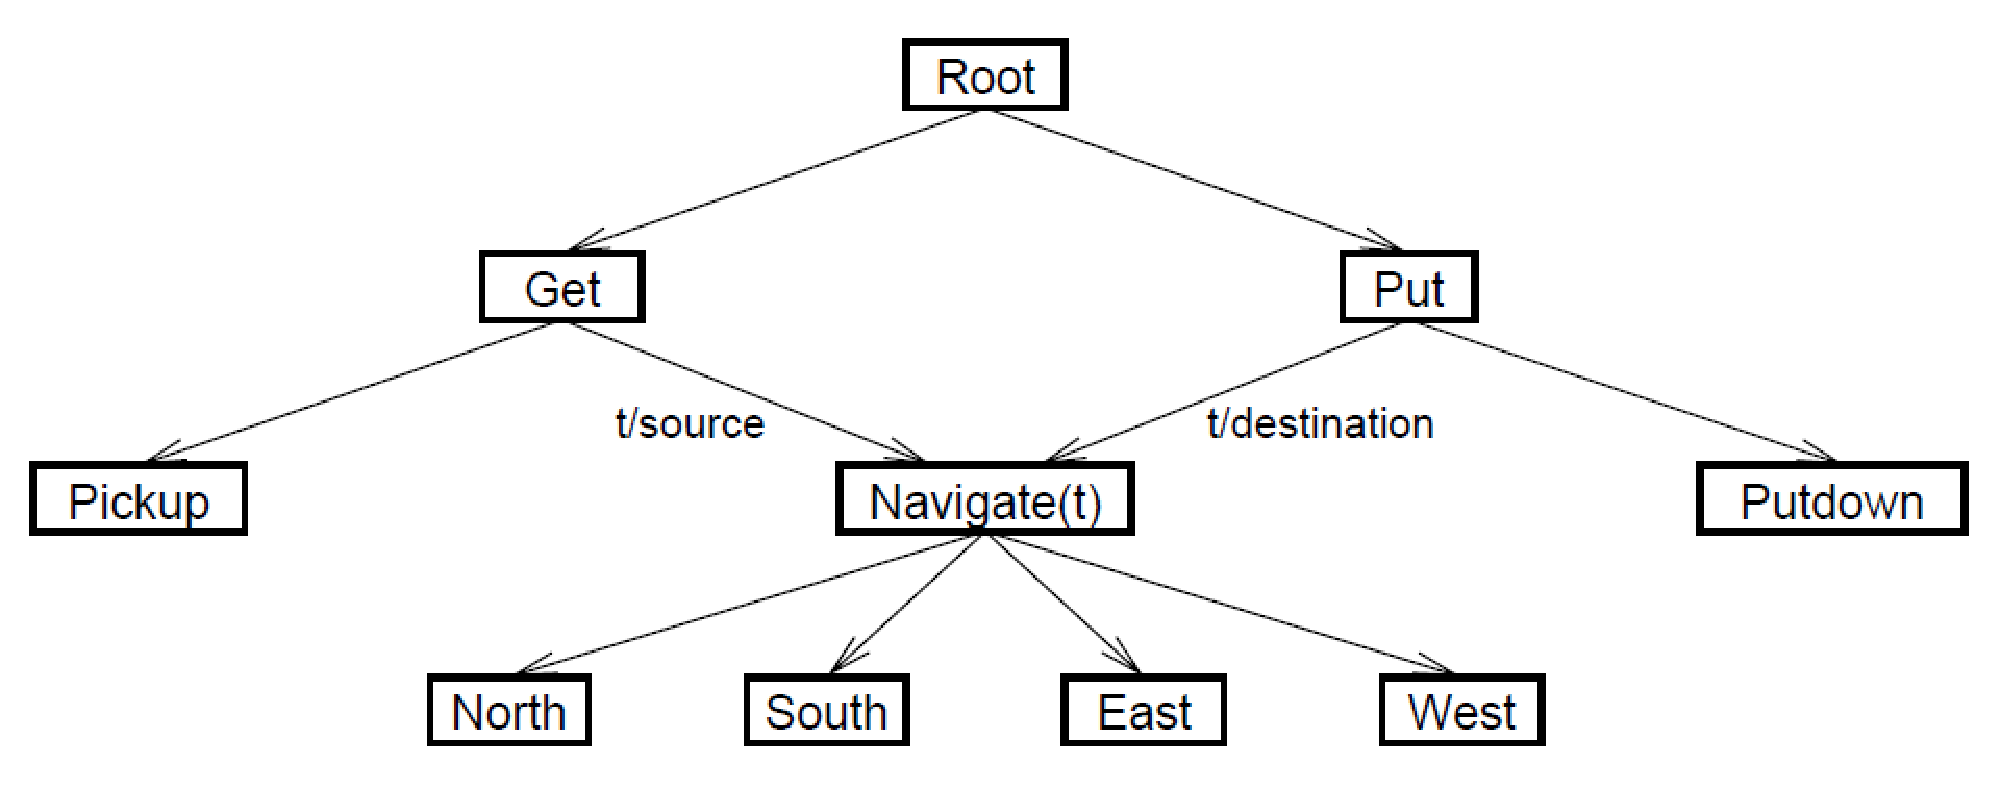
\includegraphics[width=4in] {TaxiHierarchy.eps}
\end{center}
\caption{The task hierarchy of the taxi domain \cite{MaxQJ}.}
\label{fig:taxi}
\end{figure}

%The primary contribution of this work is to show that by combining model-based and 
%model-free approaches, we can still achieve optimality even when the model is biased.

We illustrate our idea with the task hierarchy (Fig. \ref{fig:taxi}) of the taxi domain introduced by Dietterich \cite{MaxQJ}.
The taxi problem is an episodic task. For each episode, the taxi starts
at a random location. To finish the task, the taxi needs to go to the passenger's location, pick up the passenger,
go to the destination, and put down the passenger. The task can be further decomposed two subtasks: $Get$ and $Put$. 
The goal of subtask $Get$ is to move the taxi to the passenger's location and pick up the passenger. The goal of 
subtask $Put$ is to put down the passenger at the destination.

Assume the policy of subtask $Root$ is suboptimal and always invokes $Get$ even when 
the passenger is already in the taxi. Optimality can be guaranteed if subtask $Get$
learns to deliver the passenger to his destination.
Or suppose the policy of $Root$ always chooses $Put$.
If subtask $Put$ learns to pickup the passenger when he is not in the taxi, 
we will have the optimal policy because it does not matter which decision is made 
by $Root$, the passenger can always be picked up and delivered to the destination.

The above example provides two observations.
First, in order to guarantee optimality, subtasks $Get$ and $Put$ need 
to act optimally in regards to the goal of whole problem, not 
the subgoal of each subtask. It implies that we need to seek hierarchical optimality
rather than recursive optimality.

Second, optimality cannot be guaranteed without modification of the hierarchy. In the original hierarchy, 
subtask $Get$ has no access to action $Putdown$. Even though subtask $Get$ delivers the passenger to the destination,
it cannot put him down. We need to modify the hierarchy to let subtask $Get$ be
able to solve the problem on its own. A way to achieve that is to let subtask $Get$ have access
to action $Putdown$. 

%We can only guarantee optimality by adopting HORDQ for certain positions
%in the hierarchy. The "positions" are defined by the following definition:

We define which subtasks in a given hierarchy shall act optimally with the following definition:
\begin{definition}
    $C(H) = \{M_{j_1}, M_{j_2}, \dots, M_{j_k}\}$ is a leaf cover of hierarchy $H$ 
    if there is no subtask $M_i \notin C(H)$ which has access to a primitive action.
    Furthermore, $TC(H)$ is a total leaf cover if it is a leaf cover and all primitive
    actions are directly or indirectly (through child subtasks) accessible for every 
    subtask $M_i \in TC(H)$.
\end{definition}

%A leaf cover contains the subtasks which are able to solve the problem on their own.
We can always find a leaf cover for a hierarchy by including all subtasks which have access
to primitive actions. The total leaf cover can be constructed from the leaf cover by
adding the missing primitive actions.
Consider the task hierarchy in taxi domain in Figure \ref{fig:taxi},
if we add action $Pickup$ and $Putdown$ to subtask $Navigate$, 
we get a total leaf cover which consists of subtasks $Get$, $Put$, and $Navigate$.
%Another way is to let Navigate, Get and Put subtasks
%have access to all six primitive actions and include these subtasks in the total leaf cover. 

This conversion increases the exploration space because each subtask needs to explore more actions. It may increase 
the time to learn the optimal policy. However, as we show in our experiment, a good approximate model can effectively increase
the learning rate, so the time to learn the optimal policy might still decrease overall.

%There 
%It is worth noting that we can get the same optimality guarantee with any 
%hierarchical optimal learning algorithms such as HAMQ\cite{HAMQ} or tracked decomposed Q-learning\cite{HORDQ}. However, HORDQ can be easily integrated with 
%the existing MAXQ hierarchy, while the decomposed representation of Q-function is preserved.

Andre and Russell \cite{OptimalQ}\cite{HORDQ} introduced hierarchical optimal recursive decomposed Bellman equations
which extend the decomposition of MAXQ in a way that hierarchical optimality
can be guaranteed.

The Q-value is decomposed as:
\begin{align}
    \label{eq:HordQ}
    Q^{\pi}(i, s, a) = E[\sum_{t=0}^{\infty}\gamma^t r_t] &= E[\sum_{t=0}^{N_1 - 1}\gamma^t r_t] + E[\sum_{t=N_1}^{N_2 - 1}\gamma^t r_t] + E[\sum_{t=N_2}^{\infty}\gamma^t r_t]\\
                    &= Q_r^{\pi}(i, s, a) + Q_c^{\pi}(i, s, a) + Q_e^{\pi}(i, s, a),
\end{align}
where $r_t$ is the random variable of the reward that the agent receives at step $t$, $N_1$ is the number of primitive actions to finish action $a$, 
and $N_2$ is the number of primitive actions 
to finish subtask $M_i$. $ Q_r^{\pi}$ is the expected cumulative reward for executing action $a$.
$Q_c^{\pi}$ is the expected cumulative reward when subtask $M_i$ finishes after the execution of action $a$. 
$Q_e^{\pi}$ is the expected cumulative reward when the episode ends after the execution of subtask $M_i$ .

%TODO: $Q_r$ 

%Our objective is to prove that we can learn the optimal policy if we use HORDQ \cite{HORDQ} on the subtasks which 
%belong to a total leaf cover.

%The node queries its children node to get the value of $V^{\pi}(a, s)$.
$Q_r^{\pi}$ can be computed as:
\begin{equation}
    Q_r^{\pi}(i, s, a) = 
    \left\{\begin{array}{ll}
        Q_r^{\pi}(a, s, \pi_a(s)) + Q_c^{\pi}(a, s, \pi_a(s))& \mbox{if $a$ is composite} \\
        \Sigma_{s'} P(s'|s, a)R(s'|s, a) & \mbox{if $a$ is primitive} \\  
    \end{array} \right.
    \label{eq:Qr}
\end{equation}
%In our example, to compute $Q^{\pi}(MaxRoot, s, GotoExit)$, "MaxRoot" node would query 
%"MaxExit" node to get $V^{\pi}(GotoExit, s)$.

$Q_c^{\pi}$ can be computed as:
\begin{equation}
    Q_c^{\pi}(i, s, a) = \sum_{s', N} P_{S_i}^{\pi}(i, s', N|s, a)\gamma^N[Q_r^{\pi}(i, s', \pi_i(s')) + Q_c^{\pi}(i, s', \pi(s'))],
    \label{eq:Qc}
\end{equation}
where $P_{S_i}^{\pi}(i, s', N|s, a)$ is the probability that $s'$ is the first state in $S_i$ which
is encountered after the execution of action $a$ which takes exactly $N$ steps to finish. 

%Note that $P(s'|s, \pi(s))$ and $V^{\pi}(a, s)$ are provided by the child Max nodes.
And $Q_e^{\pi}$:
\begin{equation}
    Q_e^{\pi}(i, s, a) = \sum_{s', N} P_{T_i}^{\pi}(k, s', N|s, a)\gamma^N[Q^{\pi}(k, s', \pi_k(s'))],
    \label{eq:Qe}
\end{equation}
where $k$ is the index of parent subtask which invoked subtask $M_i$.

To guarantee the optimality, we cannot use the Q-value of parent subtask $M_k$ to update $Q_e^{\pi}$ of subtask $M_i$ because the 
Q-value might not be correct due to the biased model.  Instead, 
we update $Q_e^{\pi}$ with the Q-value of next subtask in $TC(H)$.
Hence, we modify equation \ref{eq:Qe} as:

\begin{equation}
    Q_e^{\pi}(i, s, a) = \sum_{s', N} P_{T_i}(i', s', N|s, a)\gamma^N[Q^{\pi}(i', s', \pi_{i'}(s')],
    \label{eq:OptQe}
\end{equation}
where $i'$ is the next subtask in $TC(H)$ that will be invoked, $P_{T_i}^{\pi}(i', s', N|s, a)$ is the probability that $s'$ is the first state in $T_i$ which
is encountered after the execution of action $a$ which takes exactly $N$ steps to finish. 
Note that the property of leaf cover ensures that we can always find such subtask $M_{i'}$ before any primitive
action is executed. %TODO: (why?).

\begin{theorem}
    Let $C(H)$ be a leaf cover of hierarchy $H$, if $Q^{\pi} = Q_r^{\pi} + Q_c^{\pi} + Q_e^{\pi}$ and
    $Q_r^{\pi}$, $Q_c^{\pi}$,and $Q_e^{\pi}$ follow equations (\ref{eq:Qr}-\ref{eq:Qc}) and (\ref{eq:OptQe}), we have $Q^{\pi}$ satisfies:
    \begin{equation*}
    Q^{\pi}(i, s, a) = 
    \left\{\begin{array}{ll}
        \sum_{s'}P(s'|s, a)[R(s'|s, a) + \gamma Q^{\pi}(i', s', \pi_{i'}(s'))], &\mbox{if $a$: primitive} \\
        Q^{\pi}(a, s', \pi_{a}(s')), &\mbox{if $a$:composite}
    \end{array} \right.
    \end{equation*}
    \label{thm:Bell}
\end{theorem}
Although we changed the formula for $Q_e^{\pi}$, the argument of Theorem 10 in \cite{HORDQ} still holds.
We do not repeat the proof here. 

%TODO: not all s are defined in Q(i, s, a) (focus on si instead of all i)
%TODO: what if pi_c_bar may change for every step?
%TODO: what if pi_c_bar is not deterministic
%TODO: write down the Q learning algorithm and the model-based one
%TODO: why Q^*(i, s, a) = Q^*(s, a) shows that hierarchical pi is the optimal policy
%TODO: any rigorous property for leaf cover?
%TODO: do I use all assumption for the theorem?
%TODO: the relationship between HORDQ and my approach
%TODO: provide the reason why we need to acceess all primitive action (because of the dumb and never learn planner)
%TODO: show that I can convert any MDP problem to hierarchy one, thus we can always combine approximated model-based approach with HORDQ.


With Theorem \ref{thm:Bell}, we can prove that the optimal policy can be learned if there exists a 
total leaf cover for the hierarchy:
\begin{theorem}
    %$\forall \pi_{N}: A_{TC} \times S \rightarrow A_{TC}$,   
    %TODO: state that the proof does not require
    Given an MDP $M$ and a hierarchy $H$ that decomposes $M$ into a finite set of subtasks $M' = \{M_0, M_1, \dots, M_n\}$,
    let $A_p$ denote the set of primitive actions for $M$, $Q^*(i, s, a)$ be the optimal Q-function for subtask $M_i$, and
    $Q^*(s, a)$ be the optimal Q-function for $M$. If $TC(H)$ is a total leaf cover of $H$,
    we have $Q^*(i, s, a) = Q^*(s, a), \forall s \in S_i, a \in A_p, M_i \in TC(H)$
    \label{thm:opt}
\end{theorem}
\textbf{Proof:} 
    Let $\pi_f: S \rightarrow A_p$ be a policy for $M$. We can construct a hierarchical policy $\pi$, such that
    $\pi_i(s) = \pi_f(s) = a$, if $a \in A_p$, $\forall M_i \in TC(H)$ (if $a$ is not directly accessible by $M_i$, we can
    let $\pi_i(s)$ be one of its composite actions).
    From Theorem \ref{thm:Bell}, we know: 
    \begin{equation}
        Q^{\pi}(i, s, a) = \sum_{s'}P(s'|s, a)[R(s'|s, a) + \gamma Q^{\pi}(i', s', \pi_{i'}(s'))].
    \end{equation}
    If $a_2= \pi_{i'}(s')$ is a composite action, we have $Q^{\pi}(i', s', a_2) = Q^{\pi}(a_2, s', \pi_{a_2}(s'))$. 
    We can keep applying the substitution until $\pi_{a_k}(s') \in A_p$, for some $k$. Since there are no
    indirect or direct recursive calls allowed in the hierarchy, the substitution can be done in finite 
    steps. Now we have:
    \begin{equation}
        Q^{\pi}(i, s, a) = \sum_{s'}P(s'|s, a)[R(s'|s, a) + \gamma Q^{\pi}(a_k, s', \pi_{a_k}(s'))].
        \label{eq:MaxIrr}
    \end{equation}
    Note that $a_k \in TC(H)$ because all subtasks which have direct access to primitive actions belong to $TC(H)$.
    By the construction of $\pi$, we have $\pi_{a_k}(s') = \pi_f(s')$.
    
    Compare (\ref{eq:MaxIrr}) to the Bellman equation of the flat MDP:
    \begin{equation}
        Q^{\pi_f}(s, a) = \sum_{s'}P(s'|s, a)[R(s'| s, a) + \gamma Q^{\pi_f}(s', \pi_f(s'))].
        \label{eq:bellman}
    \end{equation}

    Equations (\ref{eq:MaxIrr}) and (\ref{eq:bellman}) are identical except for the Q values.
    Due to the uniqueness of the Bellman equation, we have $Q^{\pi_f}(s, a) = Q^{\pi}(i, s, a), \forall s \in S_i, a \in A_p, i \in TC(H)$. 
    If $\pi_f(s) = \pi^*_f(s)$, $Q^*(s, a)$ is a solution to equation (\ref{eq:MaxIrr}). So we have $Q^*(i, s, a) \geq Q^*(s, a)$.
    Since a hierarchical policy cannot be better than an optimal policy, we have $Q^*(s, a) \geq Q^*(i, s, a)$.
    Thus we have $Q^*(i, s, a) = Q^*(s, a)$. \textbf{Q.E.D.}

Note that the above proof does not pose any constraints on the policy of subtasks $M_i \notin TC(H)$. 
If we adopt any learning algorithms for such subtasks, we still have the same optimality guarantee. 
We can compute the optimal policy using either policy iteration or value iteration algorithms. The arguments of
Theorem 11 and 13 of \cite{HORDQ} hold in our case. We do not repeat the arguments here.
 
%Because we do not usually have the complete knowledge of reward function and transition function,
%it is more desirable if we can estimate the $Q$ value in an online fashion.
The previous equations assume we have complete knowledge about the problem and can compute
the Q-value with dynamic programming. If not, we can estimate the Q-value with
the hierarchically optimal recursive Q-learning (HORDQ) \footnote{Also called ALispQ-learning in \cite{OptimalQ}} \cite{HORDQ} 
update rules:
%use temporal difference learning instead:
%TODO: the discount term compared the Bellman 
%TODO: the value iteration here!!!

\begin{equation}
    Q_r^{t+1}(i, s, a) =
    %\left\{\begin{array}{ll}
    (1 - \alpha_t)Q_r^t(i, s, a) + \alpha_t R_t(s'| s, a)   \mbox{ if $a$ is primitive} \\
    \label{eq:TdQr}
\end{equation}
%\begin{equation}
    %\tilde{Q}_r^{t+1}(i, s, a) \leftarrow
    %\tilde{Q}_r^{t}(i', s, a') + \tilde{Q}_c^{t}(i', s, a')  \mbox{if $a$ is composite} \\
    %%\end{array} \right.
    %\label{eq:TdQr}
%\end{equation}
\begin{equation}
    Q_c^{t+1}(i, s, a) =
    %\left\{\begin{array}{ll}
    (1 - \alpha_t)Q_c^t(i, s, a) + \alpha_t \gamma^N[Q_r^{t}(i', s', a') + Q_c^t(i', s', a')] \\
    \label{eq:TdQc}
\end{equation}
%\begin{equation}
    %\tilde{Q}_c^{t+1}(i, s, a) \leftarrow
    %(1 - \alpha)\tilde{Q}_c^{t}(i, s, a) + \alpha \gamma^N[\tilde{Q}_r^{t}(i', s', a')]   \mbox{if $s' \in T_i$} \\
    %%\end{array} \right.
    %\label{eq:TdQc}
%\end{equation}

\begin{equation}
    Q_e^{t+1}(i, s, a) =
    \left\{\begin{array}{ll}
    (1 - \alpha_t)Q_e^{t}(i, s, a) + \alpha_t \gamma^N[Q_e^{t}(i', s', a')]  \mbox{ if $s' \in S_i$} \\
    (1 - \alpha_t)Q_e^{t}(i, s, a) + \alpha_t \gamma^N[Q^{t}(i', s', a')]  \mbox{ if $s' \in T_i$} \\
    \end{array} \right.
    \label{eq:TdQe}
\end{equation}
where $i'$ is the index of next subtask in $TC(H)$ that will be invoked, $a' = arg max_b Q^t(i', s', b)$.

Unfortunately, the convergence of HORDQ is an open problem (Conjecture 1 of \cite{HORDQ}).
However, if we let all subtasks in $TC(H)$ have access to all primitive actions directly, 
the convergence to the optimal policy can be guaranteed. 
\begin{theorem}
    Let $TC(H)$ be a total leaf cover for a hierarchy $H$, and $Q^t = Q_r^t + Q_c^t + Q_e^t$.
    If we use equations (\ref{eq:TdQr}-\ref{eq:TdQe}) to update the Q-values for all subtasks in $TC(H)$, 
    we have $lim_{t \rightarrow \infty} Q^t(i, s, a) = Q^*(i, s, a)$
    if the following conditions hold:
    \begin{itemize}{}
    \item Every subtask in $TC(H)$ has access to all primitive actions and can only execute primitive actions
    \item A greedy in the limit with infinite exploration (GLIE) exploration policy is followed by every subtask in $TC(H)$
    \item $Var\{R_t(s' | s, a)\}$ is finite 
    \item $\sum_t \alpha_t = \infty$ and  $\sum_t \alpha_t^2 \le \infty$
    \item $0 < \gamma < 1$ or $\gamma=1$ and all policies $\pi_i$ are proper
    \end{itemize}
    %TODO: cite Neuro-Dynamic Programming 1996
%above learning algorithm will converge (with appropriately
%decaying learning rates and exploration method) to a
%hierarchically optimal policy
 
\end{theorem}
%If we let all nodes which are the parent of some primitive Max nodes to have access
%to all primitive actions, we can construct $\mathbb{C}$ by including all 
%such nodes. 
\textbf{Proof:} 
\begin{align*}
    Q^{t+1}(i, s, a) = &Q_r^{t+1}(i, s, a) + Q_c^{t+1}(i, s, a) + Q_e^{t+1}(i, s, a) \\
                     = &(1 - \alpha_t){Q}_r^{t}(i, s, a) + \alpha_t R_t(s'| s, a) \ +\\
                       &(1 - \alpha_t){Q}_c^{t}(i, s, a) + \alpha_t \gamma^N[{Q}_r^{t}(i', s', a') + {Q}_c^t(i', s', a')] \ +\\
                       &(1 - \alpha_t){Q}_e^{t}(i, s, a) + \alpha_t \gamma^N[{Q}_e^{t}(i', s', a')]\\
                      =&(1 - \alpha_t)[{Q}_r^{t}(i, s, a) + {Q}_c^{t}(i, s, a) + {Q}_e^{t}(i, s, a)] \ +\\
                       &\alpha_t[ R_t(s'| s, a) + \gamma^N[{Q}_r^{t}(i', s', a') + {Q}_c^t(i', s', a') + {Q}_e^{t}(i', s', a')]] \\
                      =&(1 - \alpha_t) {Q}^{t}(i, s, a) + \alpha_t[ R_t(s'| s, a) + \gamma^N  {Q}^{t}(i', s', a') ]
\end{align*}
    Since $a$ and $a'$ are primitive actions, the HORDQ rule identical to the standard Q-learning update rule.
    Therefore, it converges under the same condition as Q-learning. \textbf{Q.E.D.}

One of the problem of hierarchical optimal learning algorithms is that policy $\pi_i$ of subtask $M_i$
is determined by the reward of original MDP. There are no pseudo rewards which are allowed as
in MAXQ. Due to the lack of pseudo reward, each subtask $M_i$ lacks the motivation to 
pursue the subgoal defined by the hierarchy, thus it makes the hierarchical 
design useless. It is necessary to add some pseudo reward to encourage each subtask to pursue 
the subgoal. However, we cannot guarantee optimality with a nonzero pseudo reward.
A practical approach is to use positive reward to encourage the effective exploration
in the early stage, and gradually decrease it to 0. 

%The penalty term serves as a mechanism to enforce the subtask to follow the hierarchy.
%The subtask will strictly follow the subgoal defined by the hierarchy if the penalty term is large.
%On the other hand, if the penalty term is small, the subtask is more likely to go rouge and try to 
%solve the whole problem on its own. Here we have a engineering decision: if we trust our hierarchy design, 
%we should increase the penalty term to let the agent find the optimal policy as fast as it can; 
%if not, a low penalty term allows the agent to find the optimal policy when the hierarchy doesn't work.

%Here we show a way to add the pseudo reward without violating the hierarchical 
%optimal constraint:
%\begin{theorem}
    %Let $x$ be some terminal state of subtask $M_i$, $R(x)$ be the reward
    %when the agent arrives state $x$, $\tilde{R}(x) = R(x) - r$ be the pseudo reward
    %and $r$ be the penalty term.
    %If $P(x| s, \pi_i^*(s)) = 0$, we have $Q^*(i, s, \pi^*(s)) = \tilde{Q}^*(s, \tilde{\pi}(s))$.
%\end{theorem}

%The above theorem says that the optimal policy does not change 
%if some penalty is applied at some terminal states which are not part of the optimal path.


%We need the penalty for the hierarchy to work. 
%Since we do not usually know what the optimal policy is, we may add penalty term in 
%wrong states and lose the optimality. But we do not always require 


%The idea of our work is to use the approximated model-based node to 
%compute the plan for the agent, and let the hierarchical optimal model-free node
%to execute the plan. If everything works a李世光s the plan, the agent would converge to the optimal
%policy in a short time. If not (following the plan is worse than the penalty term),
%the model-free node will take control and find the optimal policy on its own.

\section{Planning with Static Assumptions}
\label{se:Model}

Based on the results of the previous section, we can safely use any approximate model-based method 
to learn the Q-values of subtasks which do not belong to $TC(H)$ without worrying
that it will violate the optimality condition. Model-based RL requires the enumeration of all possible states during the planning process.
However, it is not feasible when the state space is too large.
Previous methods (\cite{ApproxDyna}, \cite{ApproxTree}) rely on function approximation
techniques to predict the next state. Their model is biased because it is possible 
to encounter different next states given the same state and policy for a stochastic problem. If we 
predict one of them, we ignore the stochastic nature of the problem. If we predict
several, the number of states under consideration may grow exponentially with the number of simulating steps
and become intractable after a few steps.

We notice that, for some applications, there are some variables which are more important
than others. Take the mobile robot navigation problem, for example; the location of the robot 
is the key to the planning process, while the movement of other objects in the environment is less important.
Our idea is to separate the variables into planning variables 
and environment variables. During the planning process, we enumerate all possible values of the planning variables, while assuming 
the remaining environment variables are static throughout the process. 
If we limit the number of planning variables to be small, the enumeration process can be efficient.
It also simplifies the learning of the transition and reward functions, since we only need to learn
the dynamics and reward models for the planning variables.

Let state $s = (x, y)$, where $x$ consists of planning variables and $y$ consists of environment
variables. Following the MAXQ approach, we decompose the Q-function as:
\begin{equation}
    Q^{\pi}(i, x, j) = Q_r^{\pi}(i, x, j) + Q_c^{\pi}(i, x, j),
    \label{eq:biasedMaxQ}
\end{equation}
where $Q_r^{\pi}(i, x, j)$ is provided by the child subtask $M_j$.

The task of subtask $M_i$ is to compute $Q_c^{\pi}(i, x, j)$ by:
\begin{equation}
    Q_c^{\pi}(i, x, j) = \sum_{x'} P_m^{\pi}(x'|s, j)[Q_r^{\pi}(i, x', \pi_i(x')) + Q_c^{\pi}(i, x', \pi(x'))],
    \label{eq:biasedQc}
\end{equation}

With the formula above, the Q-values can be computed by dynamic programming.

For simplicity, we use the multi-time model \cite{SMDP} to model the transition function: 
\begin{equation}
    P_m(x|s, j) = \sum^{\infty}_{N=1} \gamma^N P(x, N|s, j).
    \label{eq:multiProb}
\end{equation}

$P_m(x|s, j)$ can be estimated by:
\begin{equation}
    \tilde{P}_m(x|s, j) = (1-\alpha)\tilde{P}_m(x|s, j) + \alpha [ \gamma^N \delta_{x'x}],
    \label{eq:approxP}
\end{equation}
for all $x \in S_i$, where $\delta_{x'x}=1$ if $x' = x$ and is 0 otherwise.


\section{Experimental Results}
%TODO: Say how do we update the model (just for three iteration) with Bellman equation
%TODO: say we use MaxQ for model based approach

\begin{figure}[t]
%\begin{center}
 \begin{minipage}[b]{0.5\linewidth}
    \begin{center}
    %\includegraphics[height=11em, width=6em]{eli_bend.eps}
    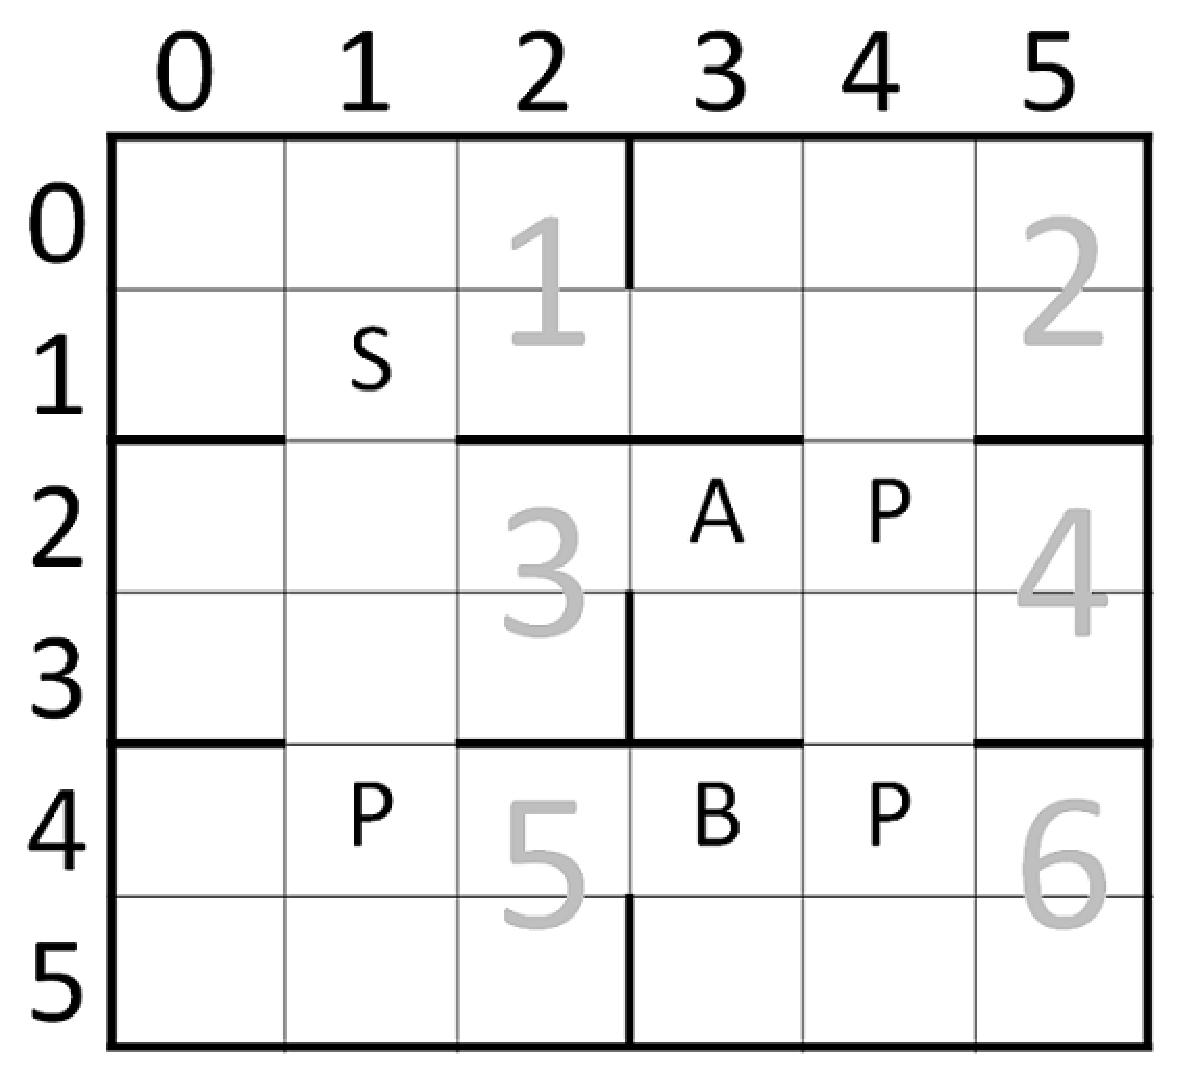
\includegraphics[width=2.0in] {BusSmall.eps}
    %\caption{(a)}
\end{center}
\end{minipage}
\begin{minipage}[b]{0.5\linewidth}
    \begin{center}
    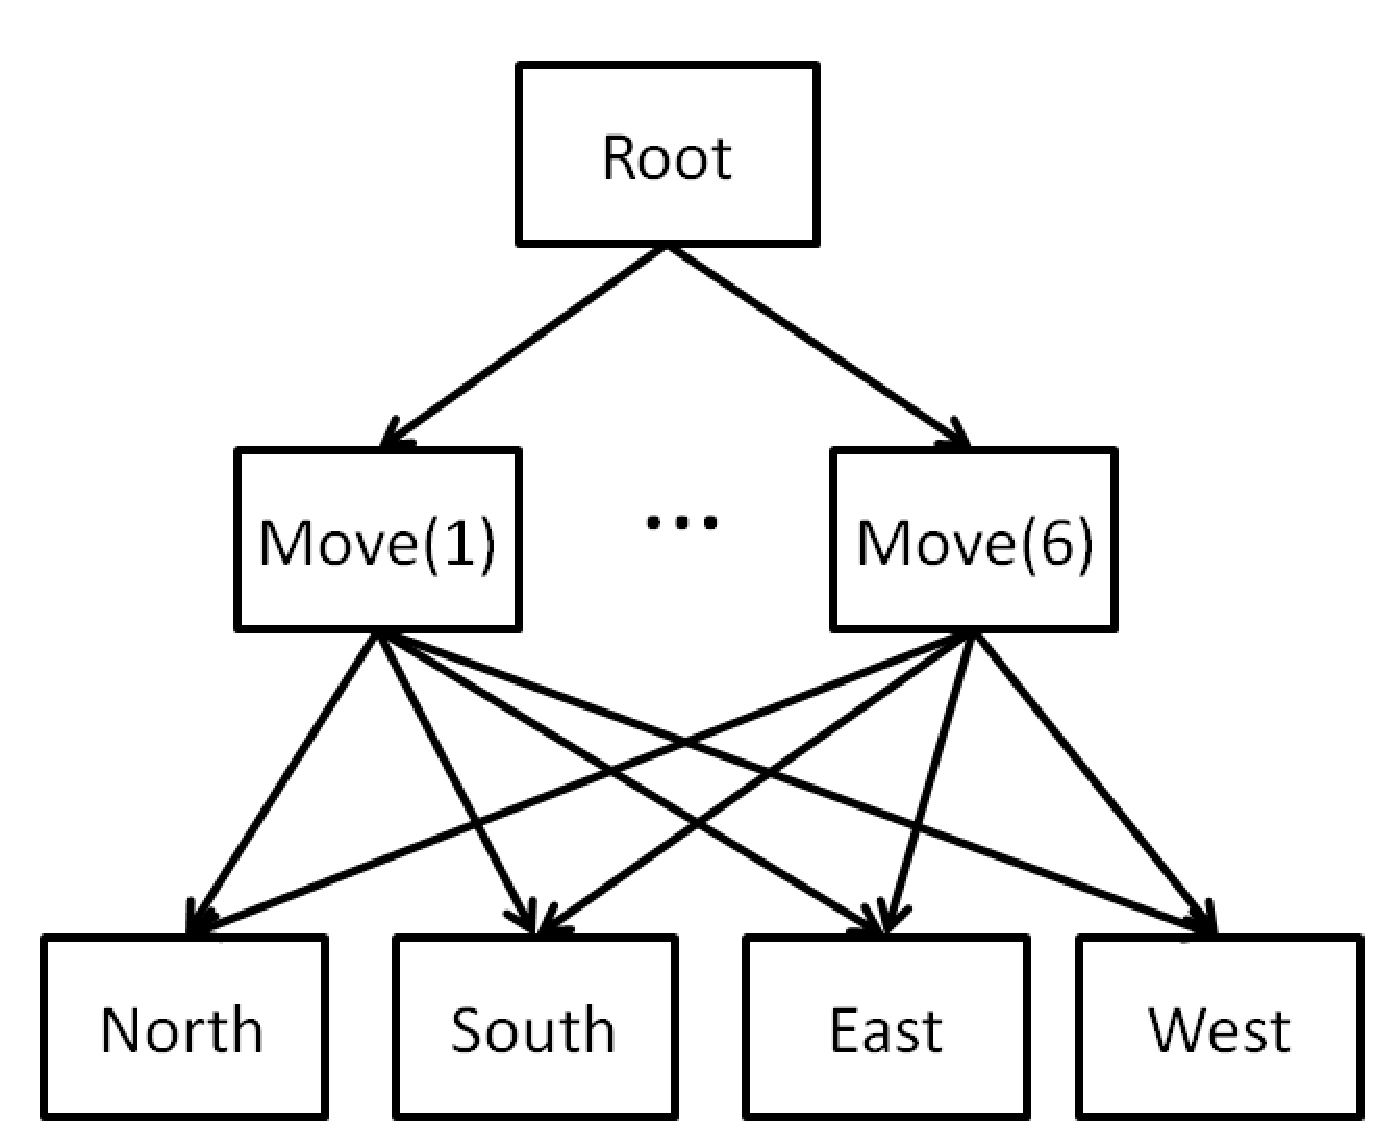
\includegraphics[width=2.0in] {BusHierarchy.eps}
\end{center}
\end{minipage}
\begin{minipage}[b]{0.5\linewidth} \centering (a) \end{minipage}
\begin{minipage}[b]{0.5\linewidth} \centering (b) \end{minipage}

%\end{center}
\caption{(a) The school bus domain (b) A task graph for the school bus domain.}
\label{fig:bus}
\end{figure}

Figure \ref{fig:bus}(a) shows the school bus domain. The school bus starts at school $S$. Its task 
is to pickup all passengers marked as $P$ and return to the school.
The bus can move North, South, East, or West. There is a reward of -1 applied for each action.
There is 0.1 probability for the bus to move in a random direction. It stays put 
when trying to cross a wall. 
The passengers are picked up automatically when the bus moves into
the location of a passenger. The passengers can be picked up in any order.
The episode ends when it finishes the task.  
There are two possible locations for road construction. They are marked as 
$A$ and $B$. If the bus passes a construction site, it will get damaged with probability 1 and has the probability
of 0.25 to break down for each step afterwards. There is a reward of -50 if the bus breaks down and the episode ends immediately. 
At the beginning of an episode, the status of the road is randomly chosen from no construction, $A$ is under construction,
or $B$ is under construction. There is a 0.05 probability for the road status to change after the episode begins.
The world is divided into six areas. There are six subtasks $Move(1), \dots,$ and $Move(6)$ which move the
bus to the corresponding area.
Subtask $Move(t)$ can only be invoked if $t$ is the adjacent area.
The subtask terminates if the bus exits the current area.
When it terminates, a pseudo-reward $\tilde{r}$ is applied if the bus arrives at designated area $t$ and 0 otherwise.
The task hierarchy is shown in Figure \ref{fig:bus}(b). 

A state can be described by the 8-tuple $(x, y, h, p_1, p_2, p_3, a, b)$, where $(x, y)$ is the location of 
bus, $h$ shows if the bus is damaged, $p_i$ indicates if the corresponding passenger has been picked up or not,
and $a$ and $b$ are binary variables which indicate the status of the construction sites.
The planning variables of our model are $\{x, y, p_1, p_2, p_3\}$, while the damage
status and road conditions are assumed to be static during the planning process.
Our model can learn that a large penalty will be received when the bus is damaged.  
%Since the damage status is assumed static during the planning process, 
However, our model cannot learn that the bus will get damaged if it passes through
a construction site. The model is certainly biased in this case, thus
it cannot learn the optimal policy. The objective of 
the experiment is to show that the optimal policy can still be learned
if we combine the model-based approach with HORDQ. 

Since the six subtasks $Move(1), \dots,$ and $Move(6)$ cover all primitive actions, they form a total leaf cover of the hierarchy.
We used HORDQ in the subtasks to guarantee the convergence to the optimal
policy. Subtask $Root$ adopted our approximate model-based method. 

%The planning variables include 
%the location of bus and the status of passengers. The environment variables are the 
%damage status of bus and the status of road. 
%TODO: total leaf cover always exist
%The world is divided by 6 areas. 

\begin{figure}[t]
%\begin{center}
 \begin{minipage}[b]{0.5\linewidth}
     \begin{center}
    %\includegraphics[height=11em, width=6em]{eli_bend.eps}
    \includegraphics[width=2.5in] {Approx.eps}
\end{center}
    %\caption{(a)}
\end{minipage}
\begin{minipage}[b]{0.5\linewidth}
     \begin{center}
    \includegraphics[width=2.5in] {Random.eps}
\end{center}
\end{minipage}
\begin{minipage}[b]{0.5\linewidth} \centering (a) \end{minipage}
\begin{minipage}[b]{0.5\linewidth} \centering (b) \end{minipage}

%\end{center}
\caption{The learning curve for the school bus domain, averaged over 400 episodes. (a) With our model-based approach. (b) With random planner.
The pseudo-reward is shown in parentheses. The parameters are $\alpha=0.1$ and $\gamma=1$. All algorithms follow an $\epsilon$-greedy exploration policy
with $\epsilon = 0.1$.}
\label{fig:res}
\end{figure}

Figure \ref{fig:res}(a) shows the learning curves with different level of pseudo-rewards.
With pseudo-reward +60, it learned a suboptimal policy because
the pseudo-reward is too large to make subtask $Move(t)$ ignore 
the penalty of breakdown. As a result, the subtask followed 
the instruction of its parent too strictly.

On the other hand, if we do not impose any pseudo-reward, 
the optimal policy can be learned, but the learning rate is
slower than SARSA(0) learning. Since the subtask has no
incentive to follow the instruction from the hierarchy, 
the learning process is similar to SARSA(0) learning 
except it has six different Q-functions to learn (one for each subtask) instead of one.
Thus it takes longer to learn the optimal policy. 

With the appropriate pseudo-reward, we can get a near-optimal policy
while the learning rate is faster than SARSA(0)
Our experiment shows that a pseudo-reward of +5 is enough to make the subtask follow 
the order of $Root$ in most of the times, but it is not enough for the subtask to ignore
the breakdown penalty. For example, when $Root$ executes $Move(4)$ to move the bus from area 
3 to area 4 and the road at location $A$ is under construction, $Move(4)$ subtask
will learn it is a bad decision with HORDQ.
Instead of moving to area 4, $Move(4)$ may move to area 1 or 5 to avoid
the breakdown penalty. In turn, $Root$ learns $Move(4)$ cannot be executed in 
such a scenario, thus it will seek an alternate plan if the same scenario
is encountered.

The combination of our approximate model-based approach and MAXQ learns 
a suboptimal policy similar to HORDQ with high pseudo-reward. MAXQ does not estimate the consequence of its action outside its own subtask, therefore
$Move(t)$ will move to area $t$ at any cost.

To simulate the performance of the combination of a poorly-approximated model-based method and 
HORDQ, we replaced our model-based approach with a random policy.
The result is shown in Figure \ref{fig:res}(b). In this case, SARSA(0) has the fastest
learning rate. It takes more time for $Move(t)$ to realize that the policy of $Root$ is bad with higher pseudo rewards.
Nevertheless, it will eventually learn a near-optimal policy.
The combination of random policy and MAXQ has the worst result.

The result shows that a good approximate model 
can help increase the learning rate with the combination of HORDQ. 
If the model is poor, HORDQ serves as a fail-safe mechanism to stop 
the agent repeating the same poor policy over and over again.
On the other hand, MAXQ learned a poor policy in both cases.  
The result suggests that in order to construct a robust HRL 
algorithm, it is beneficial to incorporate HORDQ in the hierarchy.

%On the contrary, the combination of MAXQ and a poor approximated model has
%a performance similar to random policy.

%TODO: add random agent experiment
%TODO: if I set the pseudo reward to zero, will the whole stuff breaks down again?

\section{Discussion and Future Work}
In this work, we propose an approach to combine the approximate model-based method with the model-free
method (HORDQ) under the HRL framework. We are able to show that our approach can learn the optimal
policy even when the model is biased. Furthermore, we show that the optimality is guaranteed for any subtask policy as long as 
the subtask does not belong to the total leaf cover of given hierarchy.

%TODO: STRIPS cite here
Our result suggests the possibility incorporating 
a wide range of classical planning techniques such as heuristic search or STRIPS planning
into the HRL framework without the loss of optimality.  
One future direction is to investigate the applicability of combining our method with
such techniques. 

%TODO: test on Linear approximation??
%TODO: test on Sutton's approach
%TODO: test with biased model only???

%In this work we studied both object category and instance
%recognition using the RGB-D Object Dataset [14], a large
%RGB-D (color+depth) dataset of everyday objects. Our work
%is of interest both in terms of algorithm design and of
%the empirical validations on appearance and depth cues
%for recognition. Our key insight is that because a category
%consists of different objects, there is a natural division of a
%category into subclasses, and this motivates our use of the instance
%distance. We show that by jointly learning the weights
%in this distance function, we outperform alternative state-ofthe-
%art approaches. The proposed instance distance learning
%provides a distance measure for evaluating the similarity of
%a view to a known set of objects. This information can be
%used as input to other robotics tasks, such as grasping. An
%interesting direction for future work is to treat the training
%data as an object database where grasping information is
%stored for each object. When the robot encounters an object
%in the world, it can use the instance distance classifier



{\small
\bibliographystyle{plain}
\bibliography{biblio}
}
\end{document}



\endinput
\begin{align}
    Q^\pi(i, s, a) &= Q_r^{\pi}(i, s, a) + Q_c^{\pi}(i, s, a) + Q_e^{\pi}(i, s, a) \\
    &= Q_r^{\pi}(i, s, a) + Q_c^{\pi}(i, s, a) + \sum_{s'}P(i', s', a)\gamma Q_e^{\pi}(i', s', \pi_{i'(s')}) \\
    &= \sum_{s'}P(s'|s, a)R(s'|s, a) \\
    +& \sum_{s', N}P(i', s', N| i, s, a) \gamma Q_c^{\pi}(i', s', \pi_{i'}(s')) \\
    +& \sum_{s', N}P(i', s', N| i, s, a) \gamma Q_e^{\pi}(i', s', \pi_{i'}(s')) \\
    &= \sum_{s', N}P(i', s', N| i, s, a) \gamma Q^{\pi}(i', s', \pi_{i'}(s')) \\
\end{align}
